\section{Diseño de modelo de datos para versionamiento de competencias, cursos y programas}
\subsection{Diseño del modelo de versionamiento para competencias, cursos y programas}
Al iniciar con las historias de versionamiento, se definió una tarea en la cual participaron algunos miembros de equipo y tenía como propósito principal el diseño de una lógica de negocios que permita adaptar las tablas existentes de las competencias, cursos y programas para que soporten una revisión o versionamiento de sus registros.

Como resúmen de actividades del modelo desarrollado (figura \ref{version_model}) se puede resaltar lo siguiente:
\begin{itemize}
	\item Cada tabla de cualquier entidad posee un identificador único. Las tablas entidades versionables son las de competencias, cursos, programas, y evaluaciones.
	\item Se decidió agregar una nueva columna \enquote{entity_atid} que tiene como propósito el de apuntar al origen de la versión. Por ejemplo; si el usuario crea un nuevo curso para el año lectivo, este curso tiene su identificador \enquote{course_id} y su \enquote{course_atid} apuntando a su mismo identificador por ser el origen para las versiones posteriores. Luego, se crea una nueva versión para el año posterior, esta nueva versión tiene su propio identificador pero su campo denominado como \enquote{course_atid} que apunta al primer curso creado u origen.
	\item Para hacer más sencilla la búsqueda de competencias, cursos, programas o evaluaciones actuales se agregó un campo a cada tabla identificando los actuales. Este campo denominado \enquote{is_current} o “es actual” es una bandera que indica la validez del registro.
	\item Además de registrar el origen, se registra la versión previa o de donde parte el registro con el campo \enquote{previous_entity_id}.
	\item Como cada registro de cualquier tabla ahora tiene un periodo de validez, se diseñaron tablas de relación entre cada tabla y la tabla de periodos lectivos denominada como \enquote{calendar}. Por ejemplo; \enquote{slo_term_rel} para las competencias, \enquote{new_course_term_rel} para los cursos, \enquote{asmt_term_rel} para las evaluaciones y \enquote{credential_term_rel} para los programas.
\end{itemize}

\begin{figure}
\centering
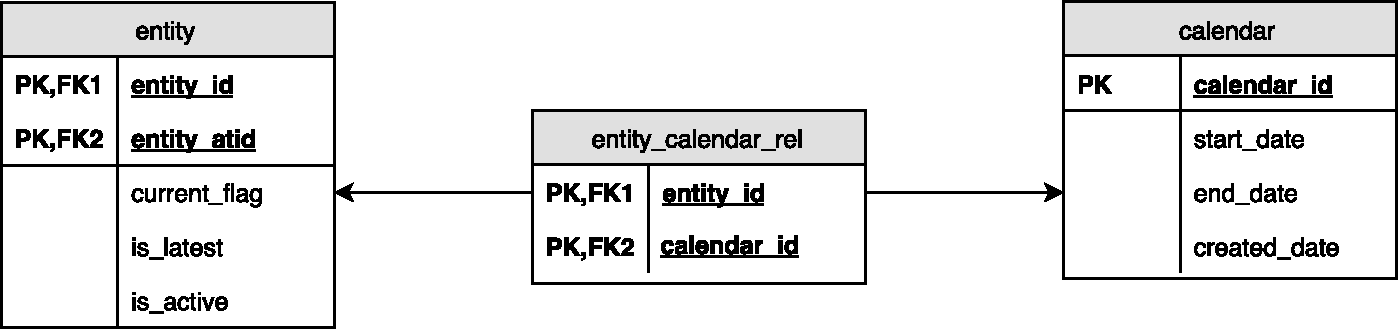
\includegraphics[width=125mm,scale=1]{Capitulos/DesarrollodelaAplicacion/Imagenes/version_model}
\caption{Modelo de datos para el versionamiento de competencias, cursos y programas.}
  \label{version_model}
\end{figure}